\documentclass{article}

\usepackage{amsmath}
\usepackage{float}
\usepackage{graphicx}

\usepackage[colorlinks=true, allcolors=blue]{hyperref}

\title{Trabalho Prático I - Introdução à Inteligência Artificial}
\author{Luís Felipe Ramos Ferreira}
\date{\href{mailto:lframos.lf@gmail.com}{\texttt{lframos.lf@gmail.com}}
}

\begin{document}

\maketitle

\section{Introdução}

O Trabalho Prático I da disciplina de Introdução a Inteligência Artificial teve como objetivo a implementação de
5 algoritmos de busca diferentes em um problema de menor caminho entre dois pontos em um mapa bidimensional.

\section{Implementação}

O projeto foi implementado utilizando C++ e Python. O código principal, que contêm a implementação dos 5 algoritmos
citados foi escrito em C++, versão 17, e está todo contido no arquivo \texttt{main.cpp}. Arquivos utilitários utilizados para
realização de \textit{benchmarks} comparativos entre os algoritmos, criação dos gráficos para análise ds dados foram criados
utilizando Python, versão 3.12.3, e os pacotes utilizados foram manejados com o gerenciador de pacotes pip.

Instruções de como executar o programa principal e os arquivos utilitários, assim como a listagem de dependências, estão
presentes no arquivo \texttt{README.md}, no diretório raiz do projeto.

Os testes apresentados na análise de resultados foram feitos em uma máquina com Ubuntu 24.04.01 e 16GB de memória RAM, na CPU
11th Gen Intel i5-11400F (12) @ 4.400GHz.


\section{Descrição dos algoritmos}

Nesta seção, é feita uma breve descrição dos algoritmos utilizados e suas principais diferenças.
Para todos eles, consideramos um \textit{branch factor} \(b\),
que a solução está no nível \(d\) e \(m\) como a profundidade máxima da árvore de busca.

\begin{itemize}
	\item \textit{Breadth First Search (BFS)}
	      A busca em largura é um algoritmo em que, a cada iteração,
	      se expande o nó mais raso ainda não expandido na busca. Em termos informais,
	      primeiro se expande a raiz, depois os sucessores da raiz, depois os sucessores
	      dos sucessores da raiz, e assim se segue. O algoritmo pode ser implementado
	      com uma fila, pois a ideia dele segue um arquitetura de FIFO (\textit{First In First Out}).
	      No algoritmo podemos fazer algo chamado \textit{Early Goal Test}, em que checamos se um nó adicionado na fila
	      já é o nó final antes de processá-lo ao sair da fila. Faz-se isso pois com isso
	      o algoritmo não irá precisar adicionar mais nós à fila e nem processar os que já estão lá se o nó final
	      já estiver pronto para ser processado.

	      \begin{itemize}
		      \item \texttt{Completo}
		      \item \texttt{Ótimo}, se e somente se o custo seja uma função
		            não decrescente da profundidade do nó (Por exemplo, na busca de menor caminho em
		            um grafo sem pesos nas arestas.).
		      \item \texttt{Complexidade}: tempo (\(\mathcal{O}(b^d)\)) e espaço (\(\mathcal{O}(b^d)\))
	      \end{itemize}

	\item \textit{Iterative Depth Search (IDS)}
	      A busca com profundidade iterativa é uma junção dos algoritmos
	      BFS e DFS. Nele, aplicamos uma busca em profundidade iterativa, isto é, a cada iteração,
	      aumentamos a profundidade permitida na busca. Nesse sentido,
	      os benefícios da BFS e da DFS são combinado.

	      \begin{itemize}
		      \item \texttt{Completo}.
		      \item \texttt{Ótimo}, considerando custo crescente como no caso da busca em largura.
		      \item \texttt{Complexidade}: tempo \(\mathcal{O}(b^d)\) e espaço
	      \end{itemize}

	\item \textit{Uniform Cost Search (UCS)}

	      O algoritmo de busca de custo uniforme é muito semelhante à BFS, mas
	      o próximo nó expandido é na verdade o nó com menor custo até o momento. Para fazer isso,
	      é necessário manter uma ordenação dos custos dos nós, e pra isso
	      podemos utilizar uma fila de prioridades ou um \textit{heap} na
	      implementação.

	      \begin{itemize}
		      \item \texttt{Completo}, se e somente se cada passo do algoritmo tem custo positivo (
		            Considerando um grafo com pesos nas arestas, se houver uma aresta com peso negativo, o algoritmo
		            não funcionaria).
		      \item \texttt{Ótimo}, uma vez que seguimos o menor custo
		      \item \texttt{Complexidade}: se \(C^*\) for a solução ótima,
		            o pior caso de tempo e espaço é \(\mathcal{O}(b^{1 + \frac{C^*}{\epsilon}})\).
	      \end{itemize}

	\item \textit{Greedy}

	      O algoritmo de busca gulosa é um tipo de algoritmo de busca com informação. Nele, expande-se o nó do espaço de busca que está mais próximo
	      do estado final de acordo com alguma função heurística definida previamente. O termo "guloso", conforme visto nos slides da disciplina, significa que o método
	      procura reduzir o custo imediato para
	      alcançar o objetivo na expansão de cada nó,
	      porém sem se preocupar com o custo total
	      do caminho. Esse algoritmo também é chamado de \textit{best first search}.

	      \begin{itemize}
		      \item \texttt{Completo}: não, ele pode entrar em um laço infinito se isso não for tratado
		      \item \texttt{Ótimo}: não
		      \item \texttt{Complexidade}: \(\mathcal{O}(b^m)\) para tempo e espaço
	      \end{itemize}

	\item \(\text{A}^*\)

	      O algoritmo \(\text{A}^*\) é um algoritmo de busca com informação que se aproveita das vantagens dos algoritmos de busca uniforme e guloso, ou seja,
	      a escolha do próximo nó a ser expandido é feita de acordo com o custo real de chegar ao nó atual mais a \textbf{estimativa} de custo de se chegar ao estado final a partir do nó atual.

	      \begin{itemize}
		      \item \texttt{Completo}
		      \item \texttt{Ótimo} se a heurística escolhida for admissível, isto é, o custo indicado pela heurística é menor ou igual
		            ao custo real para o estado final. Também é eficientemente ótimo, ou seja, expande o
		            menor número de nodos possível dentre os
		            algoritmos ótimos.
		      \item \texttt{Complexidade}: Apesar da eficiência ainda pode ser exponencial no número de nós expandidos a depender da heurística escolhida. Os nós são mantidos na memória,
		            o que também pode causar problemas.
	      \end{itemize}

\end{itemize}

\section{Modelagem}

Para fazer a leitura dos dados, uma função denominada \texttt{parse\_input\_file} foi criada. Ela recebe como entrada o caminho
para o arquivo de entrada e retorna uma matriz que representa o mapa. Cada entrada da matriz é um elemento de uma enumeração auxiliar
criada para identificar cada tipo de terreno com mais facilidade.

Para cada algoritmo foi criada uma função que recebe como entrada uma referência para a estrutura que representa o mapa e os quatro inteiros que representam
as coordenadas de começo e fim do caminho a ser percorrido pelo agente. Para padronizar a saída dos algoritmos, uma \texttt{struct} auxiliar foi criada,
denotada como \textit{SearchMethodOutput}. Ela contêm as informações de saída de um algoritmo de busca, sendo elas o custo e as coordenadas dos estados no caminho encontrado
pelo agente.

Conforme especificado na descrição dos algoritmos, cada um deles requer uma estrutura de dados específica para ser implementado, como no caso da busca em largura, que pode
ser implementada utilizando uma fila. Desse modo, a biblioteca padrão da linguagem C++ foi utilizada, pois ela contêm implementações eficientes e já prontas dessas estruturas,
as quais foram utilizadas na implementação da lógica dos algoritmos.

A função \texttt{main} identifica a partir da entrada padrão qual o algoritmo que deve ser utilizado e invoca esse procedimento
com a entrada correta após fazer a leitura do arquivo de entrada. Mais detalhes podem ser encontrados nos comentários do código no arquivo \textit{main.cpp}.

Os arquivos \textit{plot\_path.py} e \textit{plot\_expanded\_states.py} são arquivos utilitários escritos em \textit{Python} para gerar os gráficos que mostram o caminho encontrado por cada algoritmo
e os estados expandidos por eles. Por serem apenas arquivos utilitários o chatGPT foi utilizado para que eles fossem criados mais rapidamente, para que assim mais foco pudesse ser dada às análises e à implementação dos algoritmos.

\section{Heurísticas utilizadas}

Nesta seção são apresentadas as heurísticas utilizadas nos algoritmos \textit{Greedy} e \(\text{A}^*\). Em particular, a heurística escolhida para ambos os algoritmos
foi a distância \textit{Manhattan} entre dois estados/coordenadas, pois é uma heurística extremamente simples de implementar e utilizar e, além disso, muito eficiente para esse problema em particular.
Dados duas coordenadas \((x_i, y_i) e (x_f, y_f)\), a distância \textit{Manhattan} entre elas é formalmente expressada como \(|x_i - x_f| + |y_i - y_f|\).

Ela é uma heurística admissível pois o custo indicado por ela é menor ou igual ao custo real para chegar ao estado final. Isso pois o melhor caso possível, isto é, o caminho de menor custo possível
entre duas coordenadas, nesse problema, seria justamente a distância \textit{Manhtann} entre elas. Logo, a heurística é sempre menor ou igual ao custo real.

CONSISTENTE?

\section{Resultados}

Para o cálculo dos resultados, uma série de testes foi realizada. Em particular, o arquivo \textit{benchmark.py} é um código em \textit{Python} utilizado para realizar essa bateria de testes.
Como o mapa \texttt{cidade} possui dimensão 256 por 256, os testes realizados seguiram a seguinte lógica para avaliarmos como os algoritmos se comportam conforme o estado final
se distancia do estado inicial.

\begin{itemize}
	\item O estado inicial é sempre o estado com coordenada (1, 1)
	\item O estado final começa a partir do estado com coordenada (2, 2) e iterativamente aumenta com um salto de 4, indo para
	      (6, 6), (10, 10), etc.
\end{itemize}

Os resultados para cada caso de estado final foram coletados e serão apresentados nessa seção. A escolha do pulo de tamanho 4 foi feita para que os \textit{benchmarks} não demorassem muito para serem executados mas ainda assim
uma boa quantidade de informação pudesse ser coletada. Caso o estado final seja uma parede (isto é, um local que não se pode passar) apenas o ignoramos. De modo geral, isso acontece pouco e não impacta na análise.

O mapa \texttt{floresta}, por sua vez, possui uma grande quantidade de paredes, portanto sua análise foi feita de forma menos dinâmica. Para tal, alguns estados longe da origem foram escolhidos na mão.

\subsection{Custo dos caminhos encontrados}

O primeiro resultado que se mostra importante na comparação de algoritmos de busca é o costo dos caminhos encontrados. Os gráficos abaixo mostram a evolução dos custos dos caminhos para ambos os mapas disponibilizados,
conforme o estado final se distancia do inicial.

\begin{figure}[H]
	\centering
	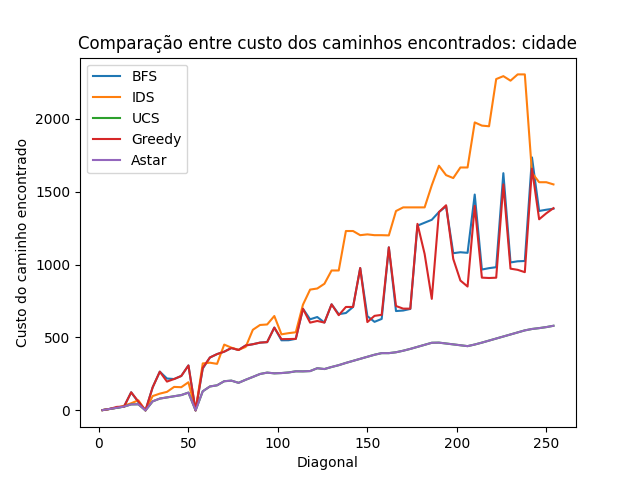
\includegraphics[width=0.8\textwidth]{../images/cidade_cost_benchmark.png}
	\caption{Comparação entre custos dos caminhos - cidade}
\end{figure}

\begin{figure}[H]
	\centering
	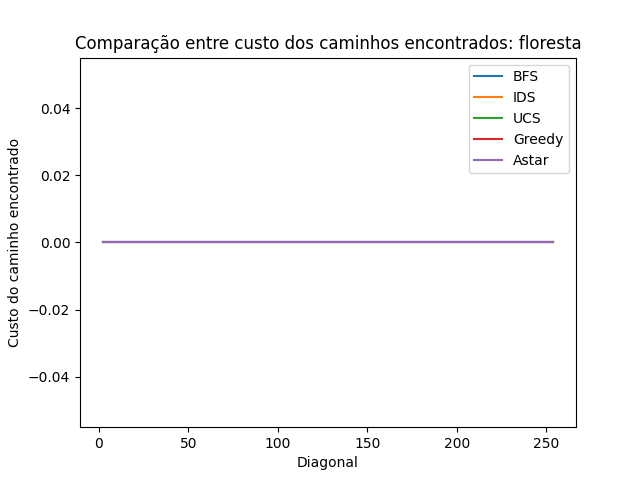
\includegraphics[width=0.8\textwidth]{../images/floresta_cost_benchmark.png}
	\caption{Comparação entre custos dos caminhos - floresta}
\end{figure}


Pode-se notar algumas coisas interessantes. Primeiramente, notamos que o custo da UCS e do \(\text{A}^*\) são iguais. Isso acontece pois ambos algoritmos são ótimos, ou seja, sempre encontram o menor caminho possível.
É importante notar também como os algoritmos guloso e a BFS apresentam custos similares, enquanto a IDS é, de longe,
o algoritmo que encontra o pior custo.

\subsection{Caminho encontrado}

O caminho encontrado é uma forma interessante de se analisar como cada algoritmo se comporta. Para a análise que será feita aqui, optou-se por imprimir o caminho encontrado por cada algoritmo entre o estado inicial
(1, 1) e o estado final (256, 256). Em particular, mostramos os caminhos encontrados por cada algoritmo no mapa \texttt{cidade}.

\begin{figure}[H]
	\centering
	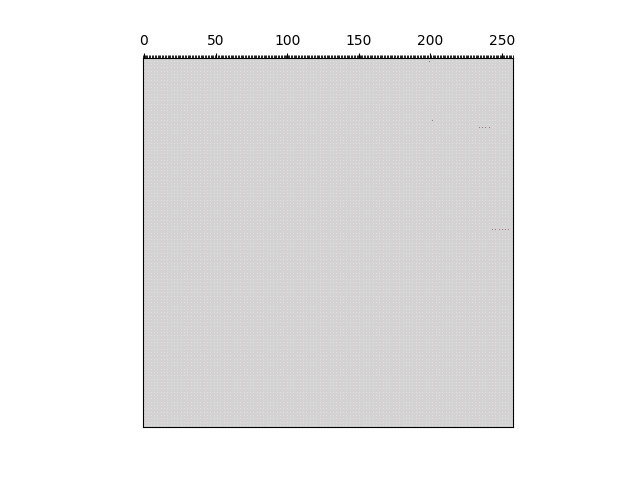
\includegraphics[width=1.0\textwidth]{../images/paths/BFS.png}
	\caption{BFS}
\end{figure}

\begin{figure}[H]
	\centering
	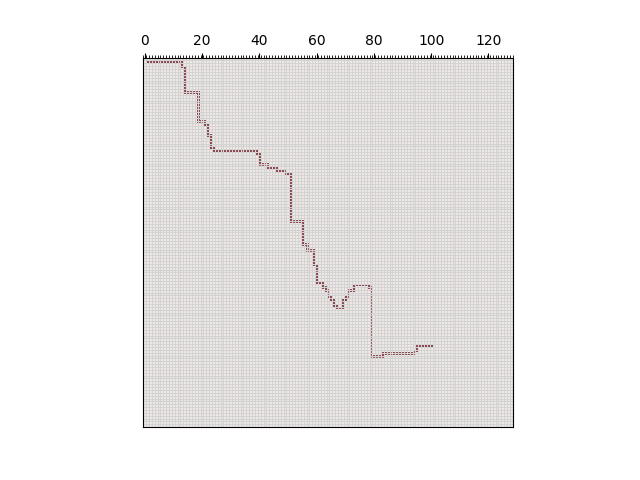
\includegraphics[width=1.0\textwidth]{../images/paths/UCS.png}
	\caption{UCS}
\end{figure}

\subsection{Número de estados expandidos}

\subsection{Tempo de execução}

Em relação ao tempo de execução, os resultados encontrados indicam exatamente o que se esperava dos algoritmos.

\section{Discussão dos resultados}

blabla

\end{document}
